\documentclass[12pt]{article}
\usepackage{amsmath} % For math blocks
\usepackage{graphicx} % For inserting images
\usepackage{quantikz} % For drawing quantum circuits and dirac notation (kets)
\usepackage{enumitem} % For using letters as list numbers
\usepackage{xcolor} % For coloring answers

\definecolor{mathRed}{RGB}{105, 0, 0} % The color used to represent the math/work to get the answers

\title{Quantum Computing Assignment \textbf{Answer Key}}
\author{Nole Stites}
\date{March 2025}

\begin{document}

\maketitle

% === QUESTION 1 ===
\section{Complexity Theory Review}
Recall that, in complexity theory, PSPACE is the class of problems solvable with polynomial space but unlimited time. Considering the complexity class diagram below, why does the class PSPACE encapsulate everything? \\

\textcolor{red}{
Accessing memory = 1 unit of time; can't access more than poly in poly-running time. Therefore, everything that takes a polynomial amount of time to run cannot access more than a polynomial amount of memory.
}
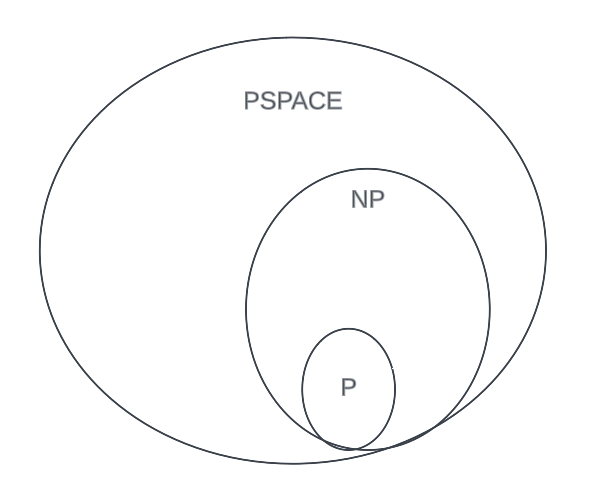
\includegraphics[]{p_np_pspace_diagram.png}

% === QUESTION 2 ===
\section{Dirac Notation}
Answer the following questions using Dirac notation. Assume that all qubits are initialized to the zero state (\ket{0}). \\
\textbf{Hint:} To verify your answers, relate them to coin flips.

\begin{enumerate}[label=\alph*]
    \item Write the state of a one-qubit computer after applying the Hadamard gate.
    \textcolor{mathRed}{
    \begin{align*}
        \ket{\psi_1} &= \ket{0} \\
        \ket{\psi_2} &= \textcolor{red}{\frac{1}{\sqrt{2}}\ket{0} + \frac{1}{\sqrt{2}}\ket{1}}
    \end{align*}
    }
    \item Write the combined state of a two-qubit computer after applying the Hadamard gate to each qubit.
    \textcolor{mathRed}{
    \begin{align*}
        \ket{\psi_1} &= \ket{0}\ket{0} \\
        \ket{\psi_2} &= (\frac{1}{\sqrt{2}}\ket{0} + \frac{1}{\sqrt{2}}\ket{1}) \cdot (\frac{1}{\sqrt{2}}\ket{0} + \frac{1}{\sqrt{2}}\ket{1}) \\
        &= \textcolor{red}{\frac{1}{2}\ket{00} + \frac{1}{2}\ket{01} + \frac{1}{2}\ket{10} + \frac{1}{2}\ket{11}}
    \end{align*}
    }
    \item Write the combined state of a three-qubit computer after applying the Hadamard gate to each qubit.
    \textcolor{mathRed}{
    \begin{align*}
        \ket{\psi_1} &= \ket{0}\ket{0}\ket{0} \\
        \ket{\psi_2} &= (\frac{1}{\sqrt{2}}\ket{0} + \frac{1}{\sqrt{2}}\ket{1}) \cdot (\frac{1}{\sqrt{2}}\ket{0} + \frac{1}{\sqrt{2}}\ket{1}) \cdot (\frac{1}{\sqrt{2}}\ket{0} + \frac{1}{\sqrt{2}}\ket{1}) \\
        &= (\frac{1}{2}\ket{00} + \frac{1}{2}\ket{01} + \frac{1}{2}\ket{10} + \frac{1}{2}\ket{11}) \cdot (\frac{1}{\sqrt{2}}\ket{0} + \frac{1}{\sqrt{2}}\ket{1}) \\
        &= \textcolor{red}{\frac{1}{2\sqrt{2}}(\ket{000} + \ket{001} + \ket{010} + \ket{011} + \ket{100} + \ket{101} + \ket{110} + \ket{111})}
    \end{align*}
    }
\end{enumerate}

% === QUESTION 3 ===
\section{Quantum Circuit}
Use the circuit below to answer the following questions.
\[
\begin{quantikz}
\lstick{\ket{q_0}} & \gate{X} & \gate{H} & \targ{} & \qw & \qw \\
\lstick{\ket{q_1}} & \qw & \gate{H} & \ctrl{-1} & \gate{H} & \qw
\end{quantikz}
\]

\begin{enumerate}[label=\alph*)]
    \item What is the depth of the circuit?
        \textcolor{red}{4}
    \item What is the space (width) of the circuit?
        \textcolor{red}{2}
    \item How many total gates are there in the circuit?
        \textcolor{red}{5}
    \item In Dirac notation, give the final state of the computer after the circuit has been executed. Assume that each qubit is initialized to the zero state.
        \textcolor{mathRed}{
        \begin{align*}
            \ket{\psi_1} &= \ket{0}\ket{0} \\ 
            \ket{\psi_2} &= \ket{1}\ket{0} \\ 
            \ket{\psi_3} &= \frac{1}{\sqrt{2}}(\ket{0} - \ket{1}) \cdot \frac{1}{\sqrt{2}}(\ket{0} + \ket{1}) \\
            &= \frac{1}{2}\ket{00} + \frac{1}{2}\ket{01} - \frac{1}{2}\ket{10} - \frac{1}{2}\ket{11} \\
            \ket{\psi_4} &= \frac{1}{2}\ket{00} + \frac{1}{2}\ket{11} - \frac{1}{2}\ket{10} - \frac{1}{2}\ket{01} \\
            \ket{\psi_5} &= \frac{1}{2}\ket{0}(\frac{1}{\sqrt{2}}\ket{0} + \frac{1}{\sqrt{2}}\ket{1}) + \frac{1}{2}\ket{1}(\frac{1}{\sqrt{2}}\ket{0} - \frac{1}{\sqrt{2}}\ket{1}) \\ &\quad - \frac{1}{2}\ket{0}(\frac{1}{\sqrt{2}}\ket{0} - \frac{1}{\sqrt{2}}\ket{1}) - \frac{1}{2}\ket{1}(\frac{1}{\sqrt{2}}\ket{0} + \frac{1}{\sqrt{2}}\ket{1}) \\
            &= \frac{1}{2\sqrt{2}}\ket{00} + \frac{1}{2\sqrt{2}}\ket{01} + \frac{1}{2\sqrt{2}}\ket{10} - \frac{1}{2\sqrt{2}}\ket{11} \\ &\quad - \frac{1}{2\sqrt{2}}\ket{00} + \frac{1}{2\sqrt{2}}\ket{01} - \frac{1}{2\sqrt{2}}\ket{10} - \frac{1}{2\sqrt{2}}\ket{11} \\
            &= \textcolor{red}{\frac{1}{\sqrt{2}}\ket{01} - \frac{1}{\sqrt{2}}\ket{11}}
        \end{align*}
        }
\end{enumerate}

% === QUESTION 4 ===
\section{Extra Credit}
Consider the 2-qubit state
\[
\ket{\phi} = \frac{1}{\sqrt{2}}\ket{00} + \frac{1}{\sqrt{2}}\ket{11}.
\]

Show that this state is entangled by proving that there are no possible values $\alpha_0$, $\alpha_1$, $\beta_0$, $\beta_1$ such that
\[
\ket{\phi} = (\alpha_0 \ket{0} + \alpha_1 \ket{1})(\beta_0 \ket{0} + \beta_1 \ket{1}).
\]
\textbf{Hint:} It may help to create a system of equations.

\textcolor{red}{
Step 1: Expand the right-hand side of the equation with FOIL
\[
\ket{\phi} = \alpha_0\beta_0\ket{00} + \alpha_0\beta_1\ket{01} + \alpha_1\beta_0\ket{10} + \alpha_1\beta_1\ket{11}
\]
Step 2: Create a system of equations for the probability amplitudes across both equations.
\begin{align*}
    \alpha_0\beta_0 &= \frac{1}{\sqrt{2}} \\
    \alpha_0\beta_1 &= 0 \\
    \alpha_1\beta_0 &= 0 \\
    \alpha_1\beta_1 &= \frac{1}{\sqrt{2}}
\end{align*}
Step 3: Observe the system of equations. For example, consider the equation $\alpha_0\beta_1 = 0$. For this to hold true, either $\alpha_0$ or $\beta_1$ must be 0. If $\alpha_0$ were 0, then the first equation $\alpha_0\beta_0 = \frac{1}{\sqrt{2}}$ would be false. If $\beta_1$ were zero, the final equation $\alpha_1\beta_1 = \frac{1}{\sqrt{2}}$ would be false. Therefore, there are no possible values $\alpha_0$, $\alpha_1$,
$\beta_0$, $\beta_1$ such that $\ket{\phi} = (\alpha_0 \ket{0} + \alpha_1 \ket{1})(\beta_0 \ket{0} + \beta_1 \ket{1})$.
}
\end{document}
